\section{Durchführung}
\label{sec:Durchführung}

\subsection{Versuchsaufbau}
Der experimentelle Aufbau ist in dem Röntgengerät integriert (siehe Abb. \ref{fig:aufbau}).
Zum wesentlichen Bestandteil des Aufbaus gehört die Kupfer-Röntgenröhre, der Plexiglas-Streuer/LiF-Kristall und das Geiger-Müller-Zählrohr.
Das Röntgengerät soll im Folgenden über einen Computer gesteuert werden.
\begin{figure}
    \centering
    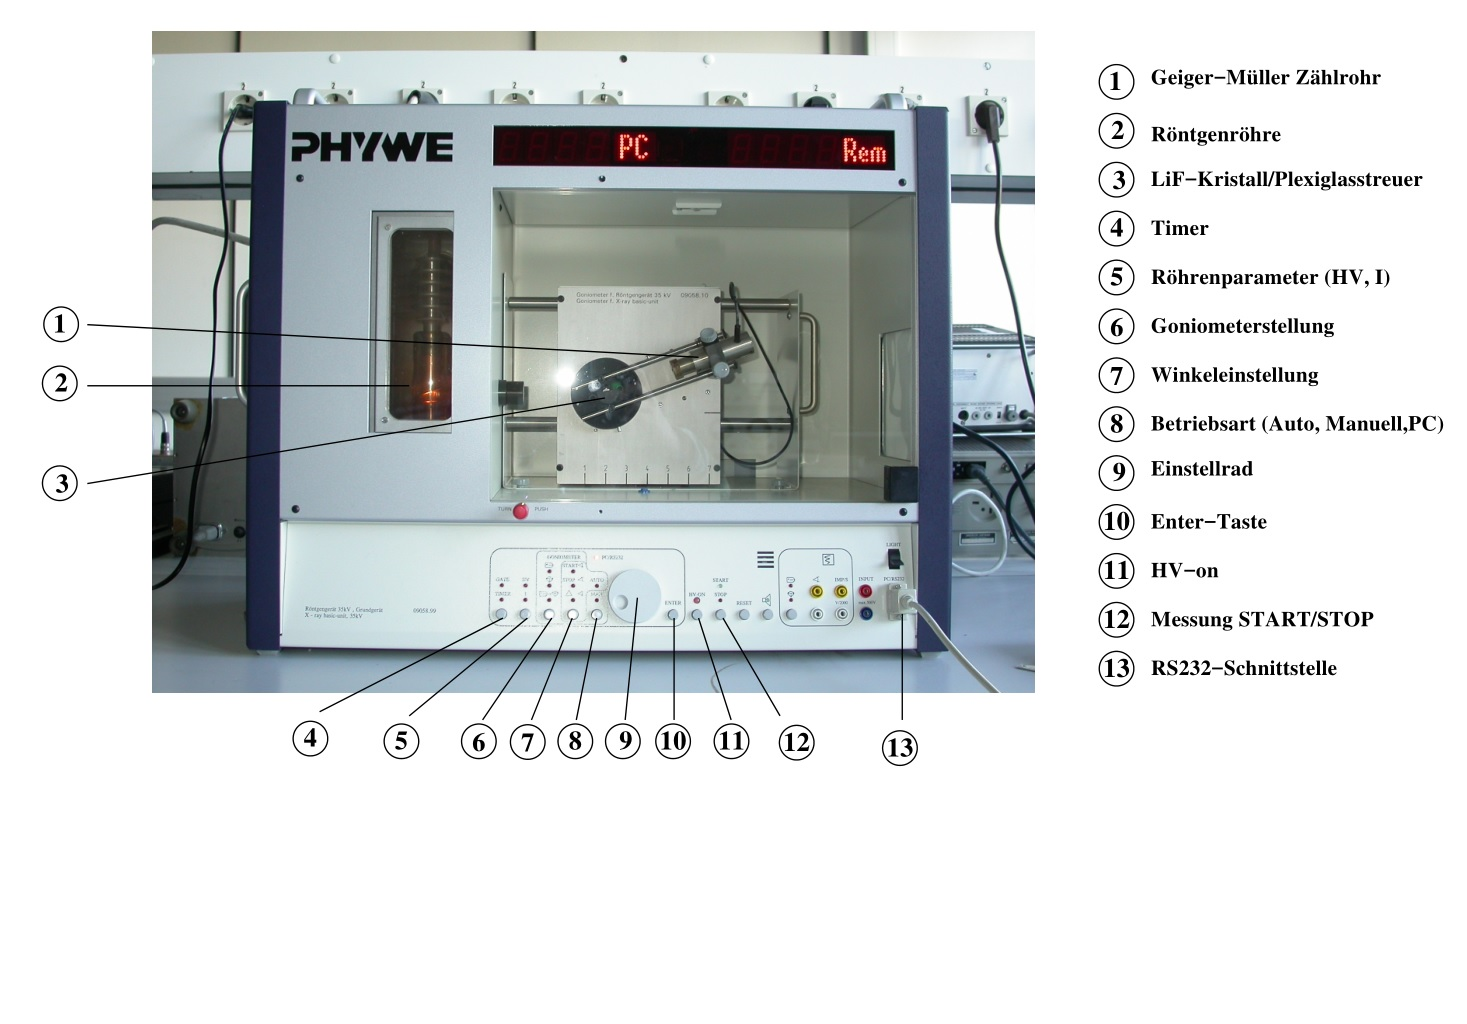
\includegraphics[width=\textwidth]{content/data/aufbau.jpg}
    \caption{Aufbau eines Röntgengeräts. \cite[3]{anleitung}}
    \label{fig:aufbau}
\end{figure}
Die Röntgenröhre soll eine Beschleunigungsspannung von $\SI{35}{\kilo\volt}$ und einen Emissionsstrom von $\SI{1}{\milli\ampere}$ erhalten.
Der LiF-Kristall und die $\SI{1}{\milli\metre}$-Blende wird in die vorgesehene Halterung gesteckt.
\FloatBarrier

\subsection{Überprüfung der Bragg Bedingung}
Der LiF-Kristall wird auf den Winkel $\theta = \SI{14}{\degree}$ gestellt.
Das Geiger-Müller Zählrohr soll in $\Delta \alpha = \SI{0.1}{\degree}$ -Schritten im Winkelbereich von $\alpha_{GM} = \SI{26}{\degree}$ bis $\alpha_{GM} = \SI{30}{\degree}$ die Intensität der Röntgenstrahlung messen.
Die Integrationszeit wird auf $\Delta t = \SI{5}{\second}$ eingestellt.

\subsection{Das Emissionsspektrum einer Cu-Röntgenröhre}
Um das Emissionsspektrum zu messen, muss im Programm der $2:1$ Koppelmodus eingeschaltet sein.
Das Röntgenspektrum soll für die Beugungsordnung $n=1$ im Winkelbereich $\theta = \SI{8}{\degree}$ bis $\theta = \SI{25}{\degree}$ in $\Delta \theta = \SI{0.1}{\degree}$ -Schritten gemessen werden.
Es wird eine Integrationszeit von $\Delta t = \SI{10}{\second}$ festgelegt.

\subsection{Das Absorptionsspektrum}
Zuerst wird ein Zinkabsorber vor das Geiger-Müller Zählrohr gesetzt und das Absorptionsspektrum in $\SI{0.1}{\degree}$ -Schritten gemessen.
Das Spektrum wird für den Zinkabsorber in dem Bereich von $\SI{18.0}{\degree}$ bis $\SI{19.5}{\degree}$ bei einer Messzeit von $\Delta t = \SI{20}{\second}$ aufgenommen.
Die Messung wird für 5 weitere Elemente wiederholt.
Der Messbereich muss jeweils angepasst werden (siehe Tab. \ref{tab:messzeit}).
\begin{table}
    \centering
    \begin{tabular}{c|cc}
    \toprule
    Element & $\theta_\text{Anfang} \,/\, \si{\degree}$ & $\theta_\text{Ende} \,/\, \si{\degree}$ \\
    \midrule
    Zink & 18.0 & 19.5 \\
    Gallium & 17.0 & 19.0 \\
    Brom & 12.8 & 14.3 \\
    Rubidium & 11.2 & 12.5 \\
    Strontium & 10.5 & 12.0 \\
    Zirkonium & 9.5 & 11.0 \\
    \bottomrule
    \end{tabular}
    \caption{Die Elemente und der Messbereich für die das Absorptionsspektrum gemessen wird.}
    \label{tab:messzeit}
\end{table}